\subsubsection{ADI and AEI Visualization}
The ADI and AEI indices measure the diversity and evenness of sounds in a sound file, usually used to draw conclusions as to the diversity of animals at the site. For these indices, a single value is used to represent their values. The algorithms used in this service provide both a right and left channel ADI and AEI value where relevant, along with band values for each frequency range tested. Thus, a single numerical value representation for single file or dataset analysis is available, along with a graph showing these values at each band range. However for comparing ADI and AEI across data sets, it may be more beneficial to use these single values to create a line graph. See the comparison section for more details on this. In addition, it is useful to compare the ADI and AEI, and when the user does \textit{both} indices on a file or data set, the service will compare them appropriately using a line graph.\\

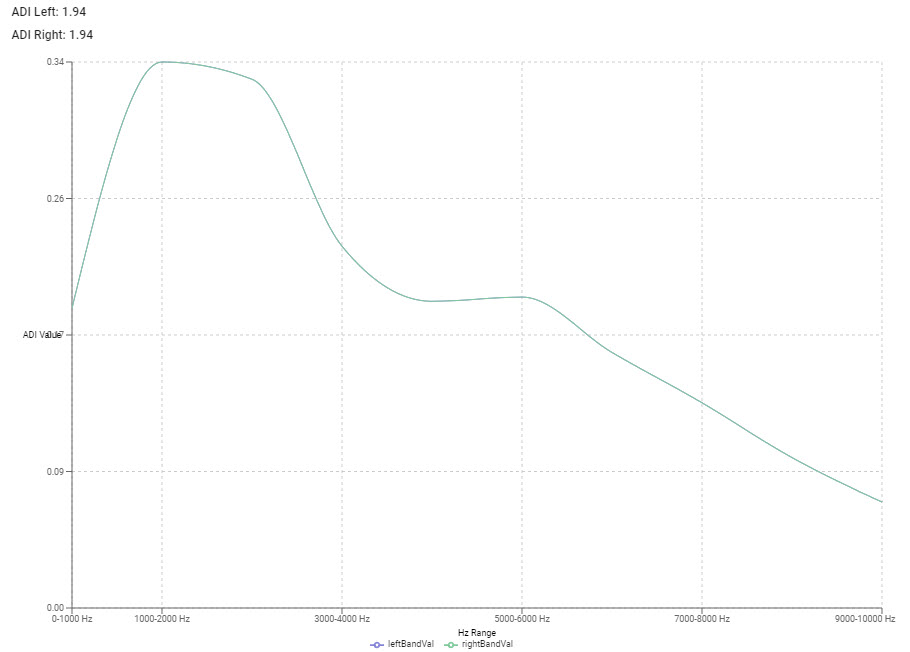
\includegraphics[width=\textwidth]{ADIgraph1}
This visualization is done on a single file using the ADI index. The X axis shows the band ranges that were determined by the user, while the Y axis shows the ADI values. This line chart also includes the ability to hover over data points to see the exact data. In addition, reference lines have been added to show the ADI value for the right and left channels, to show the average values as a baseline.
